\documentclass[dvipsnames,aspectratio=169]{beamer}
\beamertemplatenavigationsymbolsempty
\usecolortheme{beaver}
\setbeamertemplate{blocks}[rounded=true, shadow=true]
\setbeamertemplate{footline}[page number]
%
\usepackage[utf8]{inputenc}
\usepackage[english]{babel}
\usepackage{amssymb,amsfonts,amsmath,mathtext}
\usepackage{subfig}
\usepackage[all]{xy} % xy package for diagrams
\usepackage{array}
\usepackage{multicol} % many columns in slide
\usepackage{hyperref} % urls
\usepackage{hhline} %tables

%--------------------------------------------------------------------------------------
\title[\hbox to 56mm{Theme}]{Anti-Distillation: Knowledge Transfer from a Simple Model to the Complex One}
\author[K.~Petrushina]{Kseniia~Petrushina}
\institute{Moscow~Institute~of~Physics~and~Technology}
\date{\footnotesize
\par\smallskip\emph{Coauthors:} Oleg~Bakhteev, Andrey~Grabovoy, Vadim~Strijov
\par\bigskip\small 2022}
%--------------------------------------------------------------------------------------

\begin{document}

%--------------------------------------------------------------------------------------
\begin{frame}
\thispagestyle{empty}
\maketitle
\end{frame}

%--------------------------------------------------------------------------------------

\begin{frame}{Motivation}
    
    \textbf{Goal}: Adapting the \textit{student} model to more complex data using information from \textit{teacher} model.

    \bigskip

    \textbf{Challenge}: Existing \textit{teacher} model can be not suitable for new data.

    \bigskip

    \textbf{Solution}: Extend the \textit{teacher} model to get better initialization of the new model (\textit{Anti-Distillation}\footnote{Distillation -  process of transferring knowledge from a complex model to the simple model}).

\end{frame}


\begin{frame}{Distillation}
    
    \begin{center}
        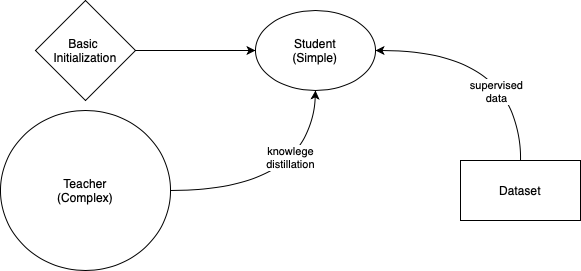
\includegraphics[width=\textwidth]{figures/distilation.png}
    \end{center}

\end{frame}


\begin{frame}{Anti-Distillation}
    
    \begin{center}
        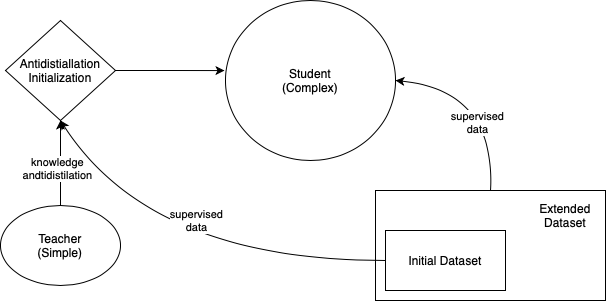
\includegraphics[width=\textwidth]{figures/andtidistilation.png}
    \end{center}

\end{frame}

%--------------------------------------------------------------------------------------

\begin{frame}{Problem statement}

    Consider two datasets
    
    $$\mathfrak{D}_1 = \{(\mathbf{x}_i, y_i)\}_{i=1}^{m_1},~\mathbf{x}_i \in \mathbb{R}^{n},~y_i \in C_1 = \{1, \dots, c_1\},$$

    $$\mathfrak{D}_2 =  \{(\mathbf{x}_i, y_i)\}_{i=1}^{m_2},~\mathbf{x}_i \in \mathbb{R}^{n},~y_i \in C_2 = \{1, \dots, c_2\}.$$
    
    $\mathfrak{D}_2$ is more complex than $\mathfrak{D}_1$.
    \bigskip
    
    Optimal parameters $\hat{\textbf{u}}$ of the teacher model $g$ on $\mathfrak{D}_1$ dataset are obtained from 
    $$\hat{\mathbf{u}} =  \underset{\mathbf{u}}{\arg\min}~\mathcal{L}_\text{ce}(\mathbf{u}, \mathfrak{D}_1) ,$$
    
    $\mathcal{L}_\text{ce}(\mathbf{u}, \mathfrak{D}_1)$ - cross-entropy loss on $\mathfrak{D}_1$.

\end{frame}

%--------------------------------------------------------------------------------------

\begin{frame}{Problem statement}

    Student model is

    \[\mathbf{f}_\text{st}: \mathbb{R}^{n} \rightarrow \Delta^{c_2},\quad \mathbf{f}_\text{st}(\mathbf{x}) = \mathbf{f}(\mathbf{x}, \hat{\mathbf{w}}),\]

    Optimization problem:

    
    \[\hat{\mathbf{w}} =  \underset{\mathbf{w}}{\arg\min}~\mathcal{L}_\text{ce}(\mathbf{w}, \mathfrak{D}^\text{val}_2),\]

    Function
    \[\boldsymbol{\varphi}: \mathbb{R}^{N_\text{tr}} \rightarrow \mathbb{R}^{N_\text{st}}\] 
    maps the teacher model parameters to student initial parameters $\mathbf{w} = \boldsymbol{\varphi}(\hat{\mathbf{u}})$.

    \newtheorem{hypothesis}{Hypothesis}
    \begin{hypothesis}
    The student models initialized by the result of applying the function $\boldsymbol{\varphi}$ to the parameters of the pre-trained teacher model is more persistent and achieve higher accuracy than models with default parameters.
    \end{hypothesis}

\end{frame}

%--------------------------------------------------------------------------------------


\begin{frame}{Problem solution}
    
    Function for weights initialization:
    
    $$\varphi(\mathbf{u}) = \underset{\mathbf{w}}{\arg\min}~\mathcal{L}(\mathbf{w}),$$
 \[\mathcal{L}(\mathbf{w}) = \lambda_1 \mathcal{L}_\text{ce}(\mathbf{w}, \mathfrak{D}_1) + \lambda_2 \mathcal{L}_2 (\mathbf{w}, \mathbf{u}) + \lambda_3 \mathcal{L}_3^\delta (\mathbf{w}, \mathfrak{D}_1) + \lambda_4 \mathcal{L}_4 \left(\displaystyle \frac{\partial^2 \mathcal{L}_\text{ce}}{\partial \mathbf{w}^2}\right)\]

    \begin{itemize}
        \item $\mathcal{L}_2 (\mathbf{w}, \mathbf{u}) = \|\textbf{u} - \textbf{Pr}[\textbf{w}]\|^2_2$  -- small difference between common weights in student and teacher.
        \item $\mathcal{L}_3^\delta (\mathbf{w}, \mathfrak{D}_1) = \displaystyle \sum \limits_{(\textbf{x}, y) \in \mathfrak{D}_1} \displaystyle \mathbb{E}_{\textbf{x}' \in U_\delta(\textbf{x})} \mathcal{L}_\text{ce}(\mathbf{w}, (\textbf{x}', y))$ -- robustness to noise with respect to input data.
        \item $\mathcal{L}_4 \left(\displaystyle \frac{\partial^2 \mathcal{L}_\text{ce}}{\partial \mathbf{w}^2}\right) = \text{tr} \left(\displaystyle \frac{\partial^2 \mathcal{L}_\text{ce}}{\partial \mathbf{w}^2}\right) $-- robustness to noise with respect to model parameters.
    \end{itemize}

\end{frame}

%--------------------------------------------------------------------------------------

\begin{frame}{Computational experiments}

\begin{columns}
\begin{column}{0.5\textwidth}
    \textbf{Data}: Fashion-MNIST dataset 
    \begin{center}
        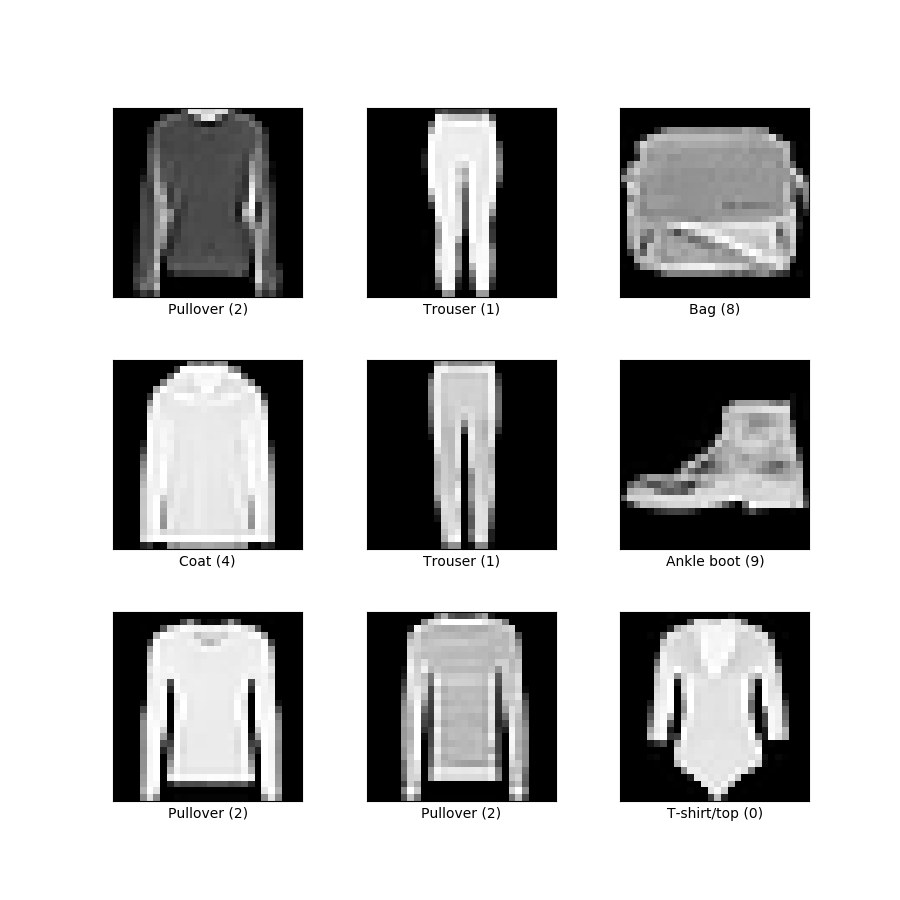
\includegraphics[width=\textwidth]{figures/fashion_mnist.png}
    \end{center}

\end{column}

\begin{column}{0.5\textwidth}
    \textbf{Model}: Multilayer perceptron

    \textbf{Baselines}: 
    \begin{itemize}
        \item Xavier initialization
        \item Transfer Learning
        \item Net2Net
    \end{itemize}

    \textbf{Quality criteria}
    \begin{itemize}
        \item Accuracy on validation set.
    
        \item Accuracy on validation set corrupted by FSGM-attack.

        \item Accuracy on validation set, provided that the model parameters are corrupted with noise: ${\mathbf{w}_\varepsilon} = \mathbf{w} + \varepsilon \boldsymbol{\xi}$, where $\boldsymbol{\xi} \sim \mathcal{N} (\mathbf{0}, \mathbf{I})$.
    \end{itemize}

    \textbf{Hyperparameter optimization}

\end{column}    
\end{columns}

\end{frame}


%--------------------------------------------------------------------------------------

\begin{frame}{Accuracy on validation set}

    \begin{columns}
        \begin{column}{0.5\textwidth}
            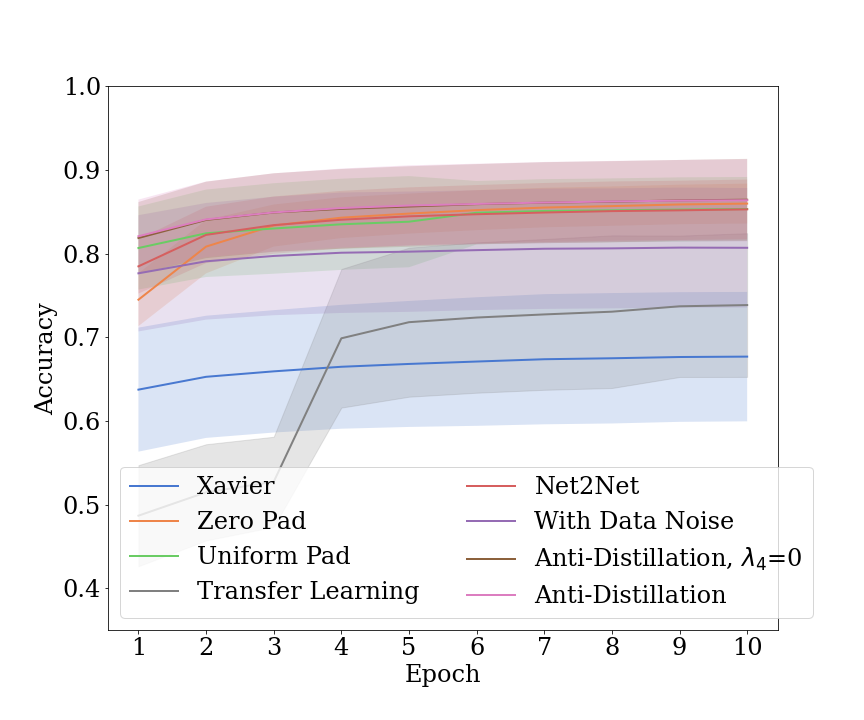
\includegraphics[width=1.2\textwidth]{figures/file.png}    
        \end{column}

        \begin{column}{0.5\textwidth}
        \begin{center}
        Anti-Distillation outperformes other methods.
        \bigskip

        \begin{tabular}{|c|c|c|c|}
            \hline Xavier & Zero & Uniform & Transfer\\
             \hline 0.68 & \textbf{0.86} & 0.85 & 0.74 \\ 
             \hline
        \end{tabular}
    
            \bigskip 

            \begin{tabular}{|c|c|c|c|}
                \hline Net2Net & Noise & AD, $\lambda_4$=0 & AD\\
                \hline 0.85 & 0.81 & \textbf{0.86} & \textbf{0.86} \\
                \hline
            \end{tabular}
        \end{center}
        
        \end{column}
    \end{columns}


\end{frame}

%--------------------------------------------------------------------------------------


\begin{frame}{Robustness to FSGM-attack}

     \begin{columns}
        \begin{column}{0.5\textwidth}
            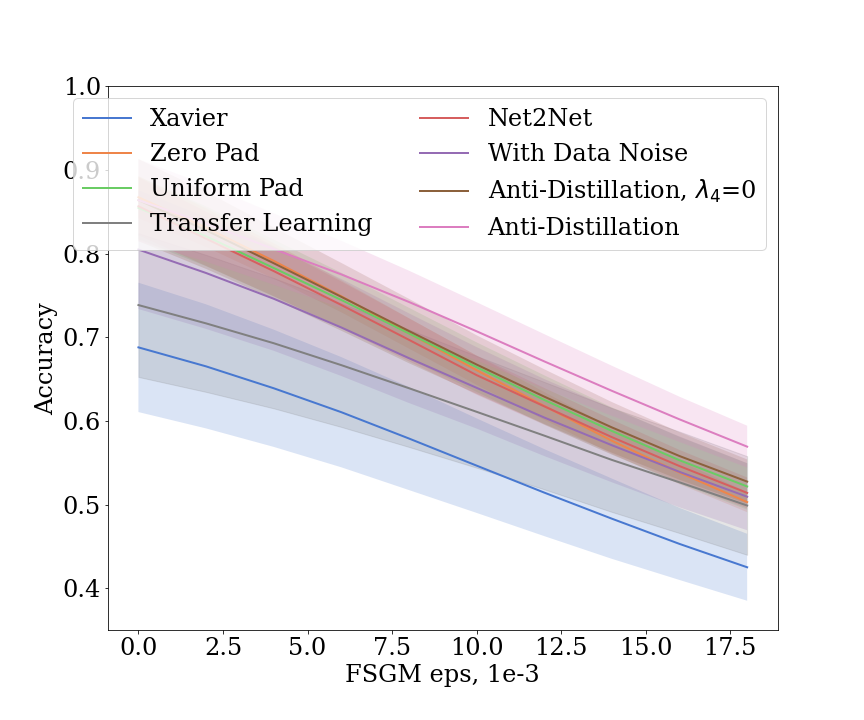
\includegraphics[width=1.2\textwidth]{figures/fsgm.png}    
        \end{column}

        \begin{column}{0.5\textwidth}
        
            \begin{center}
            Anti-Distillation outperformes other methods.
            \bigskip

            \begin{tabular}{|c|c|c|c|}
                \hline
                 Xavier & Zero & Uniform & Transfer\\
                 \hline 0.42 & 0.50 & 0.52 & 0.50 \\
                 \hline
            \end{tabular}

            \bigskip 

            \begin{tabular}{|c|c|c|c|}
                \hline Net2Net & Noise & AD, $\lambda_4$=0 & AD\\
             \hline 0.51 & 0.51 & 0.53 & \textbf{0.57} \\ 
             \hline
            \end{tabular}
            \end{center}
        \end{column}
    \end{columns}

\end{frame}

%--------------------------------------------------------------------------------------

\begin{frame}{Robustness to noise in model parameters}

    \begin{columns}
        \begin{column}{0.5\textwidth}
            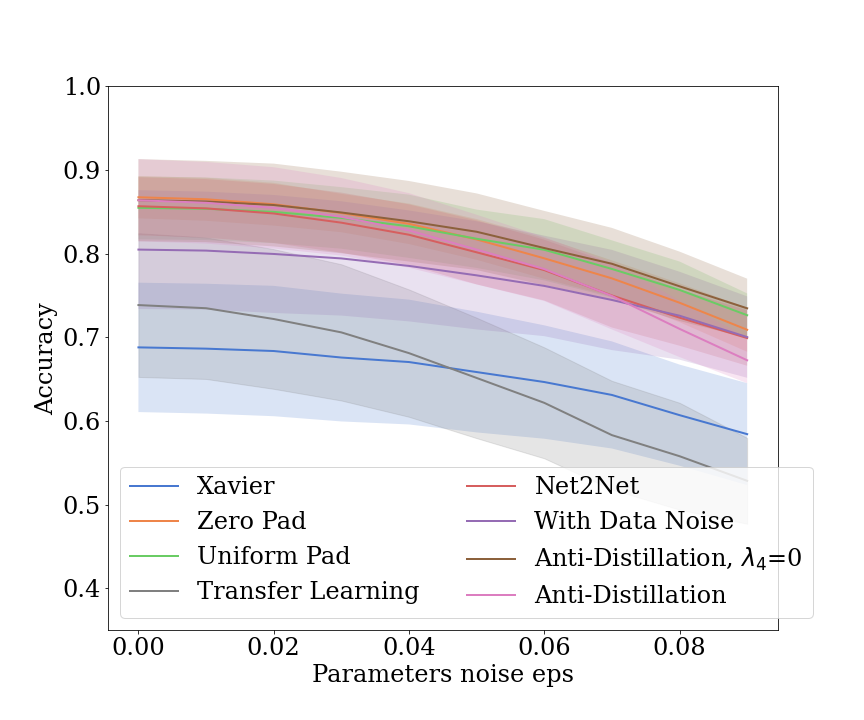
\includegraphics[width=1.2\textwidth]{figures/noise.png}    
        \end{column}

        \begin{column}{0.5\textwidth}
            \begin{center}
            Anti-Distillation outperformes other methods.
            \bigskip

            \begin{tabular}{|c|c|c|c|}
                \hline Xavier & Zero & Uniform & Transfer\\
                \hline 0.58 & 0.71 & \textbf{0.73} & 0.53 \\
                \hline
            \end{tabular}
    
            \bigskip 
    
            \begin{tabular}{|c|c|c|c|}
            \hline Net2Net &  Noise & AD, $\lambda_4$=0 & AD\\
             \hline 0.70 & 0.70 & \textbf{0.73} & 0.67 \\
            \hline
            \end{tabular}
        \end{center}
        
        \end{column}
    \end{columns}

\end{frame}

%--------------------------------------------------------------------------------------

\begin{frame}{Conclusion}
    We:
    \begin{itemize}
        \item considered the problem of the model extension to a new dataset.
        \item proposed the method for knowledge transfer from a simple model to a more complex model.
    \end{itemize}

    Anti-Distillation:
    \begin{itemize}
        \item achieved higher accuracy on \textit{more complex} dataset. 
        \item showed robustness of the Anti-Distillation to adversarial noise in input data and normal noise in model parameters.
    \end{itemize}

    \bigskip

    \textbf{Next}: other datasets, other neural network architectures.

\end{frame}

%--------------------------------------------------------------------------------------


\begin{frame}{Literature}
    \begin{itemize}
        \item Geoffrey Hinton, Oriol Vinyals, and Jeff Dean. Distilling the knowledge in a neural network, 2015.
        \item Xavier Glorot and Yoshua Bengio. Understanding the difficulty of training deep feed- forward neural networks, 2010.
        \item Tianqi Chen, Ian Goodfellow, Jonathon Shlens. Net2Net: Accelerating Learning via Knowledge Transfer, 2015.
    \end{itemize}

\end{frame}

\end{document} 